\documentclass{uimppracticas}

%Permitir cabeceras y pie de páginas personalizados
\pagestyle{fancy}

%Path por defecto de las imágenes
\graphicspath{ {./images/} }

%Declarar formato de encabezado y pie de página de las páginas del documento
\fancypagestyle{doc}{
	%Pie de Página
	\footerpr{}{}{{\thepage} de \pageref{LastPage}}
}

%Declarar formato de encabezado y pie del título e indice
\fancypagestyle{titu}{%
	%Cabecera
	\headerpr{}{}{}
	%Pie de Página
	\footerpr{}{}{}
}

\appto\frontmatter{\pagestyle{titu}}
\appto\mainmatter{\pagestyle{doc}}

\begin{document}
	
%Comienzo formato título
\frontmatter

%Portada (Centrado todo)
\centeredtitle{./images/LogoUIMP.png}{Máster Universitario en Investigación en Inteligencia Artificial}{Curso 2020-2021}{Sistemas de Recomendación}{Recomendación para grupos \\ en Python}

\begin{center}
	\large \today
\end{center}

\vspace{40mm}

\begin{flushright}
	{\bf Laura Rodríguez Navas}\\
	\textbf{DNI:} 43630508Z\\
	\textbf{e-mail:} \href{rodrigueznavas@posgrado.uimp.es}{rodrigueznavas@posgrado.uimp.es}
\end{flushright}

\newpage

%Índice
\tableofcontents

\newpage

%Comienzo formato documento general
\mainmatter

\setlength\parskip{2.5ex}

\section{Introducción}\label{introducción}

El crecimiento de Internet y de la información disponible en línea ha hecho que sea mucho más difícil extraer información útil de manera efectiva. La abrumadora cantidad de datos requiere mecanismos de filtrado de información eficientes. Uno de los sistemas utilizados para hacer frente a este problema son los sistemas de recomendación.

En este documento se describe el desarrollo práctico en Python de un sistema de recomendación. El sistema de recomendación elegido se denomina de Filtrado Colaborativo (Usuario-Usuario). La implementación se puede encontrar en~\cite{GitHubRepo}, la cual está formada por el desarrollo de un programa que implementa el sistema de recomendación de \href{https://es.wikipedia.org/wiki/Filtrado_colaborativo}{Filtrado Colaborativo}. El documento se divide en diferentes secciones donde se va describiendo paso a paso el trabajo realizado. 

En la primera parte del documento se empieza describiendo la técnica de Filtrado Colaborativo, con sus ventajas y desventajas (ver secciones~\ref{filtro_colaborativo} y~\ref{ventajas_desventajas}). El documento sigue con la descripción del conjunto de datos que usa el sistema de recomendación, y cómo podemos adquirirlo (ver sección~\ref{conjunto_datos}).

En la sección~\ref{sistema_recomendacion} del documento se describe paso a paso la implementación en Python del sistema de recomendación de Filtrado Colaborativo. En esta sección también se describe el \href{https://es.wikipedia.org/wiki/Coeficiente_de_correlaci\%C3\%B3n_de_Pearson}{coeficiente de correlación de Pearson} y porqué se ha elegido como medida para encontrar las similitudes entre los usuarios representados en el conjunto de datos y un nuevo usuario que he creado manualmente (ver sección~\ref{correlacion_pearson}). Además, también se aportan los resultados y su evaluación.

Finalmente, en la parte final del documento se añaden las conclusiones y la bibliografía.

\subsection{Filtrado Colaborativo}\label{filtro_colaborativo}

El Filtrado Colaborativo (FC) es una técnica utilizada por algunos sistemas de recomendación para predecir el grado en que, a un usuario U le gustaría un producto X. Esta técnica nos permite crear recomendaciones personalizadas, ayudar a los usuarios a encontrar productos de su interés, etc. analizando datos de muchos usuarios; asumiendo que los usuarios con gustos parecidos tienden a valorar los productos de forma similar. Es decir, si un usuario A tiene la misma opinión que un usuario B sobre un tema, el usuario A es más probable que tenga la misma opinión que el usuario B en otro tema diferente que la opinión que tendría un usuario elegido al azar. En resumen, el Filtrado Colaborativo es un método para hacer predicciones automáticas (filtrado) sobre los intereses de un usuario mediante la recopilación de las preferencias o gustos de información de muchos usuarios (colaboradores). 

Los sistemas de filtrado colaborativos basados en los usuarios, siguen una metodología que puede reducirse en los dos pasos siguientes:

\begin{itemize}
	\item En la búsqueda de usuarios que comparten los mismos patrones de valoración con el usuario activo (el usuario para el que se está haciendo la predicción).
	\item En utilizar las valoraciones por parte de aquellos usuarios afines que se encuentran en el paso 1 para calcular una predicción para el usuario activo.
\end{itemize}

En la sección~\ref{sistema_recomendacion} podremos ver detalladamente la metodología usada por el sistema de recomendación que se ha implementado en esta práctica.

\subsection{Ventajas y Desventajas del Filtrado Colaborativo}\label{ventajas_desventajas}

Algunas ventajas de un sistema de recomendación de Filtrado Colaborativo son:

\begin{itemize}
	\item Tiene en cuenta las valoraciones de otros usuarios.
	\item No necesita estudiar o extraer la información de los elementos recomendados.
	\item Se adapta a los intereses del usuario si estos cambian con el tiempo.
\end{itemize}

Algunas desventajas de un sistema de recomendación de Filtrado Colaborativo son:

\begin{itemize}
	\item Difícil de aplicar con grandes cantidades de usuarios.
	\item Difícil para encontrar suficientes vecinos para recomendar.
	\item Predice peor cuando existen pocas valoraciones.
	\item Difícil de aplicar cuando tenemos pocos datos de un nuevo producto (no ha sido valorado o ha sido poco valorado por los usuarios); o de un nuevo usuario (desconocemos sus valoraciones). Este problema se denomina el problema del \href{https://es.wikipedia.org/wiki/Arranque_en_fr\%C3\%ADo}{arranque frío}.
\end{itemize}

Para aliviar las desventajas se suele recurrir a sistemas de recomendación híbridos, que utilizan a la vez sistemas de recomendación de filtrado colaborativo y sistemas de recomendación basados en contenido. Los sistemas de recomendación basados en contenido son aquellos que tomando en cuenta algunos datos del historial del usuario intenta predecir que busca el usuario y que sugerencias similares puede mostrar. Este tipo de sistemas es uno de los que tiene mayor presencia en la actualidad.

En esta práctica no me ha parecido necesario el uso de un sistema de recomendación híbrido.

\section{Conjunto de datos}\label{conjunto_datos}

El conjunto de datos que se ha usado en esta práctica se encuentra disponible públicamente para su descarga en el siguiente enlace: \url{https://www.kaggle.com/abhikjha/movielens-100k/download}. Este conjunto de datos llamado \textit{ml-latest-small}, describe las valoraciones (entre 1 y 5 estrellas) y la actividad del etiquetado de \href{http://movielens.org}{MovieLens}~\cite{MovieLens}, un servicio de recomendación de películas. El conjunto de datos contiene 100836 valoraciones y 3683 etiquetas de 9742 películas. Los datos fueron creados por 610 usuarios que se seleccionaron al azar. Cada usuario clasificó al menos 20 películas diferentes y está representado por un identificador.

Una vez descargado el conjunto de datos podemos ver que está contenido en los archivos \textit{links.csv}, \textit{movies.csv}, \textit{ratings.csv} y \textit{tags.csv}. Aunque para esta práctica solo se utilizan los archivos \textit{movies.csv} y \textit{ratings.csv}, y estos se encuentran en la carpeta \textit{dataset} de~\cite{GitHubRepo}. Para mejorar las recomendaciones del sistema de recomendación, primero realizaremos un seguido de transformaciones en el conjunto de datos. Inicialmente empezamos cargando los archivos \textit{movies.csv} y \textit{ratings.csv} dentro de un dataframe (ver Definición~\ref{dataframe}) con el uso de la librería pandas~\cite{pandas}.

\begin{lstlisting}[language=python]
movies_df = pd.read_csv('dataset/movies.csv')
ratings_df = pd.read_csv('dataset/ratings.csv')
\end{lstlisting}

Miramos el contenido de \textit{movies\_df} para ver cómo está organizado:

\begin{table}[H]
	\centering
	\begin{tabular}{rll}
		\toprule
		movieId &                         title &                                       genres \\
		\midrule
		1 &                    Toy Story (1995) &  Adventure|Animation|Children|Comedy|Fantasy \\
		2 &                      Jumanji (1995) &                   Adventure|Children|Fantasy \\
		3 &             Grumpier Old Men (1995) &                               Comedy|Romance \\
		4 &            Waiting to Exhale (1995) &                         Comedy|Drama|Romance \\
		5 &  Father of the Bride Part II (1995) &                                       Comedy \\
		6 &                         Heat (1995) &                        Action|Crime|Thriller \\
		7 &                      Sabrina (1995) &                               Comedy|Romance \\
		8 &                 Tom and Huck (1995) &                           Adventure|Children \\
		9 &                 Sudden Death (1995) &                                       Action \\
		10 &                    GoldenEye (1995) &                    Action|Adventure|Thriller \\
		\bottomrule
	\end{tabular}
	\caption{Contenido del dataframe \textit{movies\_df} inicialmente.}
	\label{movies_df}
\end{table}

Cada película tiene un único identificador (\textit{movieId}), un título con su año de estreno y diferentes géneros. Como los años contienen caracteres \textit{unicode} y para que no haya problemas más adelante, los sacaremos de la columna de los títulos y los ubicaremos en su propia columna que nombraremos \textit{year}. Para ello, primero creamos una expresión regular para encontrar los años guardados entre paréntesis, y con la función \textit{extract} de la librería pandas los extraemos de la columna de los títulos para guardarlos en su propia columna. Después borramos los años de la columna de los títulos y con la función \textit{strip} nos aseguramos de sacar los espacios finales que pudiera haber. También eliminamos la columna de los géneros, ya que no la tendremos en cuenta en el sistema de recomendación.

\begin{lstlisting}[language=python]
regular_expression = r'\((.*?)\)'
movies_df['year'] = movies_df.title.str.lower().str.extract(regular_expression)
movies_df['title'] = movies_df.title.str.replace(regular_expression, '', regex=True)
movies_df['title'] = movies_df['title'].apply(lambda x: x.strip())
movies_df = movies_df.drop('genres', 1)
\end{lstlisting}

Vemos el resultado final:

\begin{table}[H]
	\centering
	\begin{tabular}{rll}
		\toprule
		movieId &                  title &  year \\
		\midrule
		1 &                    Toy Story &  1995 \\
		2 &                      Jumanji &  1995 \\
		3 &             Grumpier Old Men &  1995 \\
		4 &            Waiting to Exhale &  1995 \\
		5 &  Father of the Bride Part II &  1995 \\
		6 &                         Heat &  1995 \\
		7 &                      Sabrina &  1995 \\
		8 &                 Tom and Huck &  1995 \\
		9 &                 Sudden Death &  1995 \\
		10 &                    GoldenEye &  1995 \\
		\bottomrule
	\end{tabular}
	\caption{Contenido del dataframe \textit{movies\_df} final.}
	\label{movies_df_final}
\end{table}

\begin{definition}\label{dataframe}
	Un DataFrame es una estructura de datos etiquetada bidimensional que acepta diferentes tipos datos de entrada organizados en columnas. Se puede pensar en un DataFrame como una hoja de cálculo o una tabla SQL.
\end{definition}

Ahora, miraremos cómo está organizado el dataframe \textit{ratings\_df}. En este caso también eliminamos una columna, la columna \textit{timestamp}, porqué que tampoco se tendrá en cuenta en el sistema de recomendación.

\begin{lstlisting}[language=python]
ratings_df = ratings_df.drop('timestamp', 1)
\end{lstlisting}

Así es cómo queda el dataframe \textit{ratings\_df} definitivo:

\begin{table}[H]
	\centering
	\begin{tabular}{rrr}
		\toprule
		userId &  movieId &  rating \\
		\midrule
		1 &        1 &     4.0 \\
		1 &        3 &     4.0 \\
		1 &        6 &     4.0 \\
		1 &       47 &     5.0 \\
		1 &       50 &     5.0 \\
		1 &       70 &     3.0 \\
		1 &      101 &     5.0 \\
		1 &      110 &     4.0 \\
		1 &      151 &     5.0 \\
		1 &      157 &     5.0 \\
		\bottomrule
	\end{tabular}
	\caption{Contenido del dataframe \textit{ratings\_df} final.}
	\label{ratings_df_final}
\end{table}

Cada fila del dataframe \textit{ratings\_df} tiene un identificador de usuario asociado con al menos una película y una valoración de esta. Por ejemplo, en la Tabla~\ref{ratings_df_final} vemos como que el usuario 1 ha visto y valorado diferentes películas.

\section{Sistema de Recomendación}\label{sistema_recomendacion}

En esta sección describimos el sistema de recomendación, que como se ha comentado en la sección~\ref{filtro_colaborativo}, utiliza la técnica de Filtrado Colaborativo o también conocida como técnica de Filtrado de Usuario a Usuario. Con esta técnica el sistema de recomendación va a predecir recomendaciones de películas a un nuevo usuario acordes a sus gustos después de añadir nuevos datos al sistema. Para predecir las recomendaciones, el sistema de recomendación buscará las similitudes entre los datos introducidos por el nuevo usuario y los datos de los usuarios ya existentes en el sistema. Es decir, el sistema de recomendación intentará encontrar usuarios que tengan valoraciones parecidas a las del nuevo usuario, y entonces recomendarle al nuevo usuario películas acordes a sus valoraciones. Existen varios métodos para encontrar las similitudes entre los diferentes usuarios del sistema, y en el caso de este sistema, el método elegido se basa en el \href{https://es.wikipedia.org/wiki/Coeficiente_de_correlaci\%C3\%B3n_de_Pearson}{coeficiente de correlación de Pearson} (ver sección~\ref{correlacion_pearson}).

El flujo de trabajo de este sistema de recomendación sigue estos pasos:

\begin{enumerate}
	\item Crea un nuevo usuario con las películas del conjunto de datos que el usuario a mirado.
	\item Basándose en el índice de selección de películas del nuevo usuario, encuentra a sus vecinos (usuarios similares a él).
	\item Obtiene los identificadores de las películas (movieId) donde el nuevo usuario y los vecinos coinciden, es decir, obtiene los identificadores de las películas que tanto el nuevo usuario como sus vecinos hayan visto.
	\item Calcula las similitudes entre el nuevo usuario y sus vecinos.
	\item Recomienda películas al nuevo usuario según las similitudes con sus vecinos.
\end{enumerate}

Así, siguiendo el flujo de trabajo anterior, comenzamos creando un nuevo usuario a quien recomendar películas. Para ello, hemos creado el archivo \textit{new\_user.csv} dentro de la carpeta \textit{dataset}, y le hemos añadido los títulos de 100 películas elegidas aleatoriamente del conjunto de datos con una nueva valoración. En este caso, he valorado las películas según mi criterio. Este archivo se puede modificar como se desee para realizar tantas recomendaciones como se quiera, solo debemos asegurarnos de escribir bien los títulos de las películas, igual que aparecen en el archivo \textit{dataset/movies.csv}, y que valoramos las películas con un valor entre 1 y 5. A continuación, visualizamos como se organiza parte del contenido del archivo \textit{new\_user.csv}:

\begin{figure}[H]
	\centering
	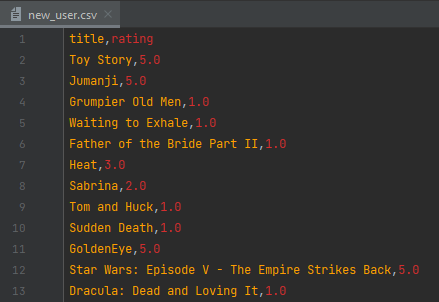
\includegraphics[scale=0.7]{images/new_user}
	\caption{Nuevo usuario del sistema.}
\end{figure}

Para finalizar con la creación del nuevo usuario, el archivo \textit{new\_user.csv} se carga dentro de un nuevo dataframe que llamaremos \textit{user\_df}:

\begin{lstlisting}[language=python]
user_df = pd.read_csv('dataset/new_user.csv')
\end{lstlisting}

Con los datos del nuevo usuario en el sistema de recomendación, extraemos los títulos de las películas que el usuario haya visto, los guardamos en la variable \textit{titles} y los unimos a los datos del usuario almacenados en el dataframe \textit{user\_df}. En este punto para ahorrar un poco de espacio de memoria, aprovechamos a eliminar la columna \textit{year} del dataframe del nuevo usuario, por qué no se utilizará más adelante en el sistema de recomendación.

\begin{lstlisting}[language=python]
titles = movies_df[movies_df['title'].isin(user_df['title'].tolist())]
user_df = pd.merge(titles, user_df)
user_df = user_df.drop('year', 1)
\end{lstlisting}

Así queda organizado el dataframe \textit{user\_df}:

\begin{table}[H]
	\centering
	\begin{tabular}{rlr}
		\toprule
		movieId &                  title &  rating \\
		\midrule
		1 &                    Toy Story &     5.0 \\
		2 &                      Jumanji &     5.0 \\
		3 &             Grumpier Old Men &     1.0 \\
		4 &            Waiting to Exhale &     1.0 \\
		5 &  Father of the Bride Part II &     1.0 \\
		6 &                         Heat &     3.0 \\
		7 &                      Sabrina &     2.0 \\
		915 &                      Sabrina &     2.0 \\
		8 &                 Tom and Huck &     1.0 \\
		9 &                 Sudden Death &     1.0 \\
		\bottomrule
	\end{tabular}
	\caption{Contenido del dataframe \textit{user\_df}.}
	\label{user_df}
\end{table}

Ahora que hemos añadido los identificadores de las películas con los datos del nuevo usuario, podemos obtener todos los usuarios que hayan visto las mismas películas, que además agruparemos por su identificador de usuario (userId).

\begin{lstlisting}[language=python]
movies = ratings_df[ratings_df['movieId'].isin(user_df['movieId'].tolist())]
users = movies.groupby(['userId'])
\end{lstlisting}

Observemos a uno de los usuarios, por ejemplo, el usuario 525.

\begin{table}[H]
	\centering
	\begin{tabular}{rrr}
		\toprule
		userId &  movieId &  rating \\
		\midrule
		525 &        1 &     4.0 \\
		525 &        2 &     3.5 \\
		525 &       34 &     3.0 \\
		525 &       39 &     4.5 \\
		525 &       48 &     3.0 \\
		525 &       62 &     3.5 \\
		525 &      107 &     3.5 \\
		525 &      150 &     4.0 \\
		525 &      223 &     3.5 \\
		525 &      377 &     3.5 \\
		525 &      480 &     4.0 \\
		525 &      595 &     3.5 \\
		525 &      915 &     3.5 \\
		525 &     1196 &     4.5 \\
		\bottomrule
	\end{tabular}
	\caption{Valoraciones del usuario 525.}
	\label{user_525}
\end{table}

El usuario 525 en total ha valorado 14 películas, 12 de las cuales no han sido valoradas por el nuevo usuario del sistema (ver Tabla~\ref{user_df}). Este hecho podría entorpecer la predicción de las recomendaciones, así que, para una mejor recomendación, donde no será necesario pasar por todos los usuarios, ordenaremos el conjunto de datos de tal forma que los usuarios que compartan la mayor cantidad de películas tengan prioridad (usuarios comunes).

\begin{lstlisting}[language=python]
common_users = sorted(users, key=lambda x: len(x[1]), reverse=True)
\end{lstlisting}

\subsection{Coeficiente de Correlación de Pearson}\label{correlacion_pearson}

Una vez encontrados los usuarios comunes o similares del sistema, podemos medir la similitud entre ellos para predecir las recomendaciones. Para ello, el sistema de recomendación buscará correlaciones entre patrones de valoración sobre las películas que han valorado los usuarios.

%HERE
En esta sección, buscamos las similitudes de todos los usuarios con el nuevo usuario para encontrar aquellos que se le parecen más. Tendremos que ver como se relacionan entre sí, y para ello usaremos el \href{https://es.wikipedia.org/wiki/Coeficiente_de_correlaci\%C3\%B3n_de_Pearson}{coeficiente de correlación de Pearson}. La fórmula para calcular este coeficiente se puede ver a continuación:

\begin{equation}\label{formula}
	r = \frac{\sum_{1}^{n} \; (x_{i} - \bar{x}) (y_{i} - \bar{y})}{\sqrt{\sum_{1}^{n}(x_{i} - \bar{x})^2} \; \sqrt{\sum_{1}^{n}(y_{i} - \bar{y})^2}}
\end{equation}

Se ha decidido usar el coeficiente de correlación de Pearson por una de sus propiedades. La propiedad dice que, si se multiplican todos los elementos por una constante distinta a cero o si se agrega cualquier constante a todos los elementos del coeficiente, este no cambia con la escala. Por ejemplo, si tenemos dos vectores $X$ e $Y$, entonces, $pearson(X,Y) = pearson(X,2\cdot Y+3)$. Esta es una propiedad muy importante en los sistemas de recomendación porqué si dos usuarios valoran dos series de elementos de manera completamente diferente, pero son usuarios muy parecidos (con ideas similares) contamos con valoraciones muy parecidas en escalas variadas.

Los valores brindados por la fórmula(\ref{formula}) pueden variar entre $r=-1$ y $r=1$, donde 1 se correlaciona directamente entre dos entidades (esto sería una correlación positiva perfecta), y -1 forma una correlación negativa perfecta. En el caso de la práctica, si el valor devuelto por la fórmula es 1 se referirá a que dos usuarios tendrán gustos parecidos, mientras que si el valor devuelto por la fórmula es -1 será lo opuesto.

A continuación, mostramos el código para calcular la correlación Pearson con la entrada del nuevo usuario, la almacenaremos en el diccionario \textit{pearsonCorrelationDict}, donde la clave será el identificador del usuario y el valor será el del coeficiente.

Elegiremos un subconjunto de usuarios para hacer las iteraciones. Este limite existe porque no queremos desperdiciar mucho tiempo pasando por cada usuario.

\begin{lstlisting}[language=python]
pearsonCorrelationDict = {}

for name, group in user_groups:     # For each user
	
	# Sorting the current user in such a way that the values don't get mixed up later
	user = group.sort_values(by='movieId')
	movies = user_df.sort_values(by='movieId')
	
	# Get the number of elements (N) for the formula
	nRatings = len(user)
	
	# Set ratings for movies in common in a list
	temp_df = movies[movies['movieId'].isin(user['movieId'].tolist())]
	tempRatingList = temp_df['rating'].tolist()
	
	# Set user ratings in a list
	tempGroupList = user['rating'].tolist()
	
	# Calculate the Pearson Correlation between two users, x and y
	Uxx = sum([i ** 2 for i in tempRatingList]) - pow(sum(tempRatingList), 2) 
		/ float(nRatings)
	Uyy = sum([i ** 2 for i in tempGroupList]) - pow(sum(tempGroupList), 2) 
		/ float(nRatings)
	Uxy = sum(i * j for i, j in zip(tempRatingList, tempGroupList)) - sum(tempRatingList)  
	* sum(tempGroupList) / float(nRatings)
	
	# If the denominator is nonzero, then we divide, otherwise the correlation is 0
	if Uxx != 0 and Uyy != 0:
		pearsonCorrelationDict[name] = Uxy / sqrt(Uxx * Uyy)
	
	else:
		pearsonCorrelationDict[name] = 0
\end{lstlisting}

Guardamos el resultado en un nuevo dataframe.

\begin{lstlisting}[language=python]
pearson_df = pd.DataFrame.from_dict(pearsonCorrelationDict, orient='index')
pearson_df.columns = ['similarityIndex']
pearson_df['userId'] = pearson_df.index
pearson_df.index = range(len(pearson_df))
\end{lstlisting}

\newpage

\subsection{Resultado y Evaluación}



Vemos el resultado:

\begin{table}[h]
	\centering
	\begin{tabular}{rr}
		\toprule
		similarityIndex &  userId \\
		\midrule
		0.171034 &     414 \\
		0.401235 &     599 \\
		0.203293 &       6 \\
		0.210447 &     474 \\
		0.353077 &     274 \\
		\bottomrule
	\end{tabular}
	\caption{Contenido del dataframe \textit{pearson\_df}.}
	\label{pearson}
\end{table}

Ahora obtenemos los 50 primeros usuarios más parecidos:

\begin{lstlisting}[language=python]
topUsers = pearson_df.sort_values(by='similarityIndex', ascending=False)[0:50])
\end{lstlisting}

\begin{table}[h]
	\centering
	\begin{tabular}{rr}
		\toprule
		similarityIndex &  userId \\
		\midrule
		1.0 &     551 \\
		1.0 &     513 \\
		1.0 &     409 \\
		1.0 &     257 \\
		1.0 &     335 \\
		\bottomrule
	\end{tabular}
	\caption{Los 50 primeros usuarios más parecidos.}
	\label{usuarios_parecidos}
\end{table}

Recomendemos películas al nuevo usuario puntuando a los usuarios elegidos para todas las películas. Haremos esto tomando el peso promedio de los ratings de las películas utilizando la correlación Pearson. Pero para hacer esto, primero necesitamos que los usuarios vean las películas en nuestro \textit{pearson\_df} a partir del dataframe de valoraciones y luego guardar su correlación en una nueva columna llamada similarityIndex. Estos se logra juntando estas dos tablas de debajo.

\begin{lstlisting}[language=python]
topUsersRating = topUsers.merge(ratings_df, left_on='userId', right_on='userId', how='inner')
\end{lstlisting}

\begin{table}[h]
	\centering
	\begin{tabular}{rrrr}
		\toprule
		similarityIndex &  userId &  movieId &  rating \\
		\midrule
		1.0 &     551 &       47 &     4.5 \\
		1.0 &     551 &      110 &     3.5 \\
		1.0 &     551 &      260 &     3.5 \\
		1.0 &     551 &      293 &     4.5 \\
		1.0 &     551 &      296 &     3.5 \\
		\bottomrule
	\end{tabular}
	\caption{Los 50 primeros usuarios más parecidos.}
	\label{usuarios_parecidos}
\end{table}

Ahora todo lo que se necesita hacer es multiplicar el puntaje de la película por su peso (El índice de similitud), luego se suman los nuevos puntajes y dividen por la suma de los pesos.
Esto se logra sencillamente multiplicando dos columnas, luego agrupando el dataframe por la columna movieId y luego dividiendo dos columnas:
Aqui se muestra la idea de todos los usuarios similares respecto de las películas candidatas para el usuario ingresado:

\begin{lstlisting}[language=python]
topUsersRating['weightedRating'] = topUsersRating['similarityIndex'] * topUsersRating['rating']
tempTopUsersRating = topUsersRating.groupby('movieId').sum()[['similarityIndex', 'weightedRating']]
tempTopUsersRating.columns = ['sum_similarityIndex', 'sum_weightedRating']
\end{lstlisting}

\begin{tabular}{rr}
	\toprule
	sum\_similarityIndex &  sum\_weightedRating \\
	&                     \\
	\midrule
	9.903247 &           40.868223 \\
	2.453957 &            9.295957 \\
	1.654654 &            4.463961 \\
	2.415235 &            4.745706 \\
	1.866025 &            7.464102 \\
	\bottomrule
\end{tabular}

Se crea un dataframe vacío
Ahora se toma el promedio ponderado

\begin{lstlisting}[language=python]
recommendation_df = pd.DataFrame()
recommendation_df['weighted average recommendation score'] = tempTopUsersRating['sum_weightedRating'] / \
tempTopUsersRating['sum_similarityIndex']
recommendation_df['movieId'] = tempTopUsersRating.index
\end{lstlisting}

\begin{tabular}{rr}
	\toprule
	weighted average recommendation score &  movieId \\
	&          \\
	\midrule
	4.126750 &        1 \\
	3.788150 &        2 \\
	2.697822 &        3 \\
	1.964904 &        5 \\
	4.000000 &        6 \\
	\bottomrule
\end{tabular}


Luego, ordenemos y veamos las primeras 20 películas que el algoritmo recomendó:




Después de obtener las recomendaciones vamos a valorarlas. 

\newpage

\section{Conclusiones}

Automatizar la creación del archivo \textit{dataset/user\_ratings.csv}.

El enlace al vídeo debéis incluirlo en la memoria. Trabajo práctico: la idea es que vayáis explicando el porqué de las decisiones que habéis tomado (qué me llevó a utilizar unos determinados hiperparámetros, por qué he utilizado esta manera de medir la calidad de la solución,...) y hagáis un razonamiento sobre los resultados obtenidos.

Ahora, calculemos el coeficiente de correlación de Pearson entre el nuevo usuario y el resto de los usuarios del conjunto de datos. El resultado lo vamos a almacenar en un diccionario, donde la clave es el identificador del usuario y el valor es el coeficiente.


\newpage

\renewcommand{\refname}{Bibliografía}
\bibliographystyle{unsrt}
\bibliography{biblio}
	
\end{document}
